\documentclass[letterpaper,11pt]{article}

% Soporte para los acentos.
\usepackage[utf8]{inputenc}
\usepackage[T1]{fontenc}
% Idioma español.
\usepackage[spanish,mexico, es-tabla]{babel}
% Soporte de símbolos adicionales (matemáticas)
\usepackage{multirow}
\usepackage{amsmath}
\usepackage{amssymb}
\usepackage{amsthm}
\usepackage{amsfonts}
\usepackage{mathtools}
\usepackage{latexsym}
\usepackage{enumerate}
\usepackage{ragged2e}
\usepackage{listings}
\usepackage{xcolor}
\usepackage{graphicx}
\usepackage{hyperref}
\usepackage[caption=false]{subfig}
\newcommand{\subsubsubsection}[1]{\paragraph{#1}\mbox{}\\}
\setcounter{secnumdepth}{4}
\setcounter{tocdepth}{4}
% Modificamos los márgenes del documento.                                       %
\usepackage[lmargin=2cm,rmargin=2cm,top=2cm,bottom=2cm]{geometry}

\definecolor{codegreen}{rgb}{0,0.6,0}
\definecolor{codegray}{rgb}{0.5,0.5,0.5}
\definecolor{codepurple}{rgb}{0.58,0,0.82}
\definecolor{backcolour}{rgb}{0.95,0.95,0.92}

\lstdefinestyle{mystyle}{
    backgroundcolor=\color{backcolour},   
    commentstyle=\color{codegreen},
    keywordstyle=\color{magenta},
    numberstyle=\tiny\color{codegray},
    stringstyle=\color{codepurple},
    basicstyle=\ttfamily\footnotesize,
    breakatwhitespace=false,         
    breaklines=true,                 
    captionpos=b,                    
    keepspaces=true,                 
    numbers=left,                    
    numbersep=5pt,                  
    showspaces=false,                
    showstringspaces=false,
    showtabs=false,                  
    tabsize=2
}

\lstset{style=mystyle}

\title{Facultad de Ciencias, UNAM \\ Redes Neuronales \\ 
       Fake News Detection Dataset}
\author{Rubí Rojas Tania Michelle}
\date{12 de junio de 2020}

\begin{document}
\maketitle

\section{Introducción}

Si bien es cierto que internet ha permitido el intercambio de conocimiento a una 
escala con la que generaciones previas sólo podían soñar, también ha fundamentado
lo que el ensayista \textit{Jonathan Swift} escribió en $1710$:

\begin{center}
    \textbf{"La falsedad vuela y la verdad viene cojeando tras ella."}
\end{center}   

En Estados Unidos, por ejemplo, una investigación del \textit{Pew Centre} reveló
que el $62\%$ de los estadounidenses adultos reciben noticias a través de las 
redes sociales, de manera que es \textbf{cada vez más probable que más de 
nosotros estemos viendo -y creyendo- información que no sólo no es precisa, 
sino que a veces es totalmente inventada}.

Actualmente existen cientos de sitios web de noticias falsas, desde los que 
imitan diarios reales, hasta sitios de propraganda gubernamental, y otras que se 
mueven por la fina línea que divide la sátira con la desinformación. 
\begin{figure}[ht]
    \centering
    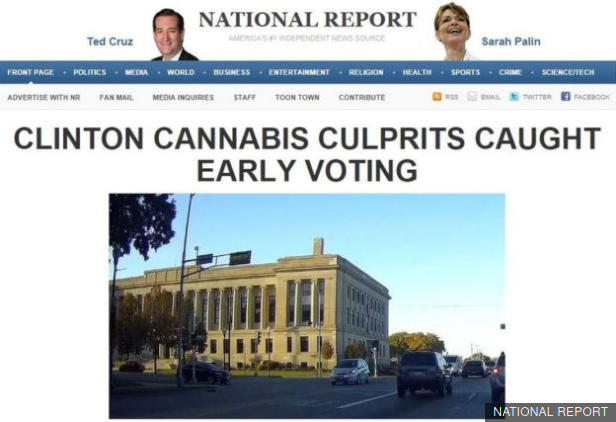
\includegraphics[width=0.4\textwidth]{imagenes/national.png}
    \caption{National Report. Sitio web dedicado a la difusión de 
             \textit{fake news}}
\end{figure}    

La principal razón por la que existen las noticias falsas es para desinformar a
la población, ya sea para fines políticos o económicos. En el primer caso, las 
noticias intentan manipular el debate público a favor de determinados intereses 
políticos, mientras que en el segundo caso, se tratan de operaciones comerciales
que buscan generar el tráfico a partir de contenidos falsos, y sobre todo, 
titulares sensacionalistas a los que la gente les da \texttt{clic}, pero cuya 
información relacionada no tiene sentido o relevancia alguna.

Ahora bien, ¿por qué es importante combatir las noticias falsas? Un motivo 
importante es que la información es esencial para las sociedades democráticas:
difundir información falsa, imprecisa o errónea atenta contra ese derecho y 
afecta la toma de decisiones con fundamento por parte de los ciudadanos. En 
otras palabras, afecta directamente la democracia. Por esta razón, es un 
deber de los ciudadanos revisar (o verificar) la calidad de los contenidos que 
consume y comparte. 

Por otro lado, sabemos que hoy en día existe una cantidad exorbitante de 
información, por lo que puede ser complicado encontrar la \textit{verdad}. 
También existe mucho sesgo de confirmación ya que mucha gente quiere probar que 
su visión del mundo es la apropiada y correcta; es decir, lo que para algunas 
personas es verdad, para otros no lo es. Esta cuestión abre un gran debate, por 
eso es importante que construyamos un criterio propio para así formar nuestro 
concepto de \textit{verdad}.
\begin{figure}[ht]
    \centering
    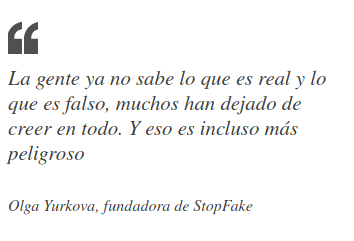
\includegraphics[width=0.4\textwidth]{./imagenes/frase.png}
\end{figure}    

\section{Objetivo}
\begin{center}
    \texttt{"Dada una noticia, queremos saber si es real o falsa."}
\end{center}

\section{Métodos}
\subsection{Conjunto de Datos}
El conjunto de noticias que utilizaremos se obtuvo del sitio web \textit{Kaggle}
\begin{center}
    \url{https://www.kaggle.com/c/fake-news/data}
\end{center}

el cual contiene dos archivos:
\begin{enumerate}
    \item \textit{train.csv}

    Contiene un conjunto de datos para entrenamiento con los siguientes 
    atributos:
    \begin{itemize}
        \item \textbf{id}: el \textit{id} único de la noticia.
        \item \textbf{title}: el título de la noticia.
        \item \textbf{author}: el autor de la noticia.
        \item \textbf{text}: el texto de la noticia (podría estar incompleto).
        \item \textbf{label}: la etiqueta que clasifica la notica como 
        \textsc{real} $(0)$ o \textsc{fake} $(1)$.  
    \end{itemize}

    \item \textit{test.csv}

    Contiene un conjunto de datos con los mismos atributos que el archivo 
    anterior, pero sin \textit{label}. 
\end{enumerate} 

\newpage
\subsection{Preprocesamiento de Datos}

Los datos contenidos en el archivo \textit{train.csv} se pueden ver de la 
siguiente forma:
\begin{figure}[h!]
    \centering
    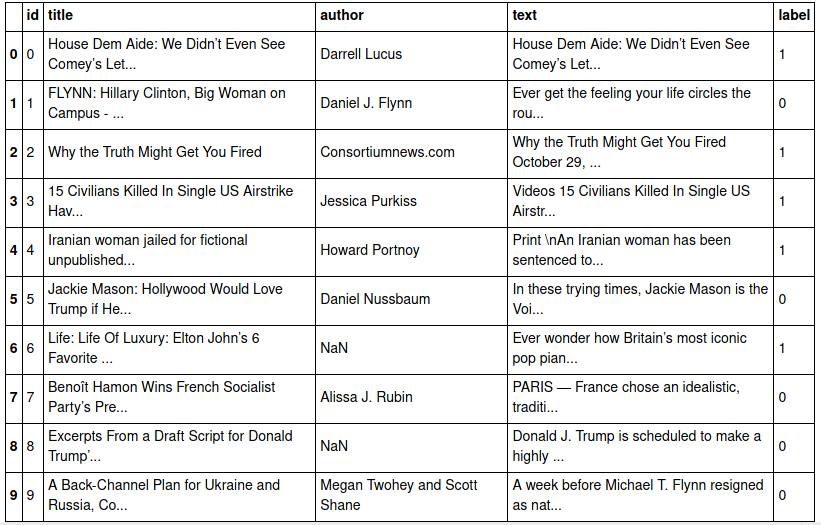
\includegraphics[width=1\textwidth]{imagenes/dataframe.png}
    \caption{DataFrame con las 10 primeras noticias}
    \label{fig: dataframe1}
\end{figure}

Renombraremos el atributo \textit{label} (para evitar confusiones por mi
parte), de manera que la etiqueta $0$ la cambiamos por \textsc{real} y la 
etiqueta $1$ la cambiamos por \textsc{fake}.

\begin{figure}[ht!]
    \centering
    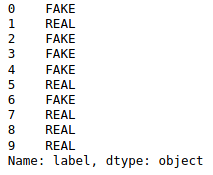
\includegraphics[width=0.3\textwidth]{./imagenes/labels.png}
    \caption{Etiquetas de las 10 primeras noticias}
\end{figure} 

Dividimos nuestro conjunto de datos con un split del $75-25$ para entrenamiento 
y prueba. 

\begin{lstlisting}[language = Python]
X_train, X_test, y_train, y_test = train_test_split(df['text'], 
                                                    labels, 
                                                    test_size = 0.25, 
                                                    random_state = 7)
\end{lstlisting}

\newpage
Un \texttt{TfidVectorizer} se encarga de \textit{vectorizar} un texto. 
\begin{itemize}
    \item \texttt{TF (Term Frequency)}: es el número de veces que una 
    palabra aparece en un documento. Un valor más alto significa que un término 
    aparece más a menudo que otros, y por lo tanto, el documento es un buen 
    candidato cuando el término es parte de los términos de búsqueda.

    \item \texttt{idf (Inverse Document Frequency)}: las palabras que ocurren 
    muchas veces en un documento, pero también muchas veces en muchos otros,
    pueden ser irrelevantes. Los \texttt{IDF} son una medida de la importancia
    de un término en todo el corpus. 
\end{itemize}

El \texttt{TFidVectorizer} convierte una colección de documentos en bruto en 
una matriz de caracterísiticas \texttt{TF-IDF} (contiene las palabras más 
relevantes dentro de la colección de documentos).

Ahora bien, inicializamos un \texttt{TfidVectorizer} con palabras de stop  del 
idioma inglés (ya que las noticias se encuentran escritas en este idioma) y una
frecuencia de documento máxima de $0.7$ (los términos con una frecuencia más 
alta serán descartados). Las palabras stop son las palabras más comúnes dentro 
del idioma que deben ser filtradas antes de procesar los datos del lenguaje 
natural. 

\begin{lstlisting}[language = Python]
# Inicializamos un TfidfVectorizer. 
v = TfidfVectorizer(stop_words = 'english', max_df = 0.7)
\end{lstlisting}

Luego, entrenamos y transformamos el \texttt{vectorizer} en un conjunto de 
entrenamiento; y transformamos el \texttt{vectorizer} en un conjunto de prueba.
\begin{lstlisting}[language = Python]
# Entrenamos y transformamos el conjunto de entrenamiento.
v_train = v.fit_transform(X_train.apply(lambda x: np.str_(x))) 

# Transformamos el conjunto de prueba.
v_test = v.transform(X_test.apply(lambda x: np.str_(x)))
\end{lstlisting}

\subsection{Plan de Acción}
Para darle una solución a nuestro objetivo, utilizaremos dos \textit{modelos}
de clasificación diferentes: un perceptrón multicapa y el algoritmo de 
clasificación Pasivo-Agresivo.

\subsubsection{Perceptrón Multicapa}

\subsubsubsection{Arquitectura}
La arquitectura utilizada para nuestra red neuronal es:
\begin{itemize}
    \item Capa de entrada: Tendremos $5$ neuronas, una por cada columna de
    nuestro conjunto de datos. 

    \item Capa oculta: Tendremos cuatro capas ocultas con dos neuronas cada 
    una. Esta elección la hice basándome en el método \textit{prueba y error}, 
    ya que estuve probando con varias arquitecturas para la capa oculta, y 
    ésta en particular me pareció rápida en comparación a las otras 
    arquitecturas que probé. 

    \item Capa de salida: Tendremos dos neuronas, ya que se trata de una 
    clasificación binaria.
\end{itemize}

\newpage
\subsubsubsection{Implementación}

\begin{lstlisting}[language = Python]
# Arquitectura.
mlpc = MLPClassifier(max_iter = 1000, 
                     learning_rate_init = 0.0001, 
                     hidden_layer_sizes = (2, 4))
\end{lstlisting}

\begin{lstlisting}[language = Python]
# Entrenamos nuestro perceptron.
mlpc_entrenamiento = mlpc.fit(v_train, y_train)

# Predecimos en el conjunto de prueba.
mlpc_prediction = mlpc.predict(v_test)

# Obtenemos la precision.
score_mlp = accuracy_score(y_test, mlpc_prediction)
print(f'Precision: {round(score_mlp * 100, 2)}%')
\end{lstlisting}

\begin{verbatim}
    Precisión: 95.77%
\end{verbatim}

\subsubsection{Algoritmo Pasivo-Agresivo}

\subsubsubsection{¿Cómo funciona?}

Los algoritmos Pasivo-Agresivo son una familia de algoritmos de aprendizaje 
en línea (tanto para la clasificación como para la regresión) propuestos
por \textit{Creammer at al}. 

Un algoritmo Pasivo-Agresivo funciona genéricamente con esta regla de 
actualización:
\begin{equation*}
    \begin{cases}
        \overline{w_{t+1}} 
        = argmin_{\bar{w}} \frac{1}{2} \| \overline{w} -
        \overline{w_t}\|^2 + C \xi^2 \\ 
        L(\bar{w}; x_t, y_t) \leq \xi 
    \end{cases}
\end{equation*}

Para comprender esta regla, supongamos que la variable $\xi = 0$ (y $L$ está 
restringida a ser $0$). Si se presenta una muestra $x(t)$, el clasificador usa 
el vector de peso actual para determinar el signo. Si el signo es correcto, 
la función de pérdida es $0$ y el argumento es $w(t)$. Esto significa que el 
algoritmo es \textbf{pasivo} cuando se produce una clasificación correcta. 
Supongamos ahora que ocurrió una clasificación errónea:
\begin{figure}[h]
    \centering
    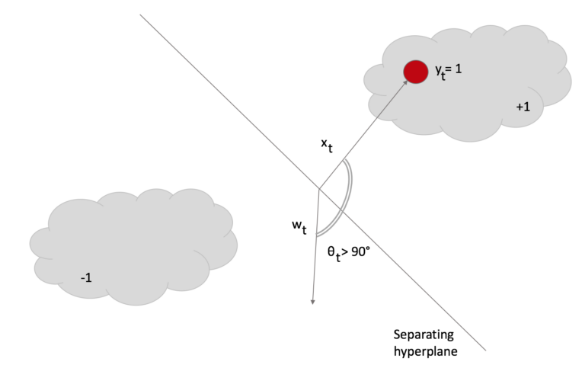
\includegraphics[width=0.4\textwidth]{./imagenes/pa1.png}
\end{figure}    

El ángulo $\theta > 90^{\circ}$, por lo tanto, el producto escalar es negativo 
y la muestra se clasifica como $-1$, sin embargo, su etiqueta es $+1$. En este 
caso, la regla de actualización se vuelve muy \textbf{agresiva} porque busca
una nueva $w$ que debe estar lo más cerca posible que la anterior (de lo 
contrario, el conocimiento existente se pierde inmediatamente), pero debe 
satisfacer $L = 0$ (en otras palabras, la clasificación debe ser correcta). 

La introducción de la variable $\xi$ permite tener márgenes blandos (como en 
$SVM$) y un grado de tolerancia controlado por el parámetro $C$. En particular,
la función de pérdida debe ser $L \leq \xi$, lo que permite un error mayor. 
Los valores más altos de $C$ producen una agresividad más fuerte (con el 
consiguiente mayor riesgo de desestabilización en presencia de ruido), mientras 
que los valores más bajos permiten una mejor adaptación. De hecho, este tipo 
de algoritmos, cuando trabajan en línea, debe hacer frente a la presencia de 
muestras ruidosas (con etiquetas incorrectas). Es necesaria una buena 
robustez; de lo contrario, los cambios demasiado rápidos produce las 
consiguientes tasas de clasificació errónea más altas.

Después de resolver ambas condiciones de actualización, obtenemos la regla de 
actualización de manera cerrada:
\begin{equation*}
    \overline{w_{t+1}} = \overline{w_t} +
    \frac{max(0, 1 - y_t (\overline{w^T} \cdot \overline{x_t}))}
         {\| x_t \|^2 + \frac{1}{2C}} y_t \overline{x_t}
\end{equation*}

Esta regla confirma nuestras expectativas: el vector de peso se actualiza con
un factor cuyo signo está determinado por $y(t)$ y cuya magnitud es proporcional
al error. Tengamos en cuenta que si no hay una clasificación errónea, la fracción
se hace cero, entonces $w(t+1) = w(t)$, mientras que, en caso de clasificación 
errónea, $w$ rotará hacia $x(t)$ y se detendrá con una pérdida $L \leq \xi$. 
En la siguiente figura, el efecto se ha marcado para mostrar la rotación, sin 
embargo, normalmente es lo más pequeño posible.
\begin{figure}[h]
    \centering
    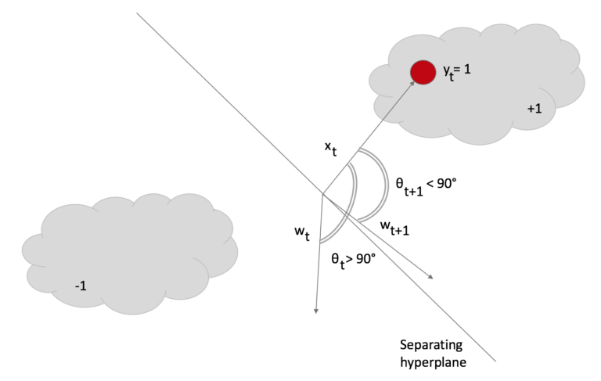
\includegraphics[width=0.4\textwidth]{./imagenes/pa2.png}
\end{figure} 

Después de la rotación, $\theta < 90^{\circ}$ y el producto escalar se vuelve 
negativo, por lo que la muestra se clasifica correctamente como $+1$. 

\subsubsubsection{Implementación}

\begin{lstlisting}[language = Python]
# Inicializamos un PassiveAggressiveClassifier.
pac = PassiveAggressiveClassifier(max_iter = 100)

# Entrenamos nuestro clasificador.
entrenamiento = pac.fit(v_train, y_train)

# Predecimos en el conjunto de prueba.
prediction_pac = pac.predict(v_test)

# Obtenemos la precision.
score = accuracy_score(y_test, prediction_pac)
print(f'Precision: {round(score * 100, 2)}%')
\end{lstlisting}

\begin{verbatim}
    Precisión: 96.4%
\end{verbatim}

\section{Resultados}

Partiéndo del hecho de que las precisiones obtenidas fueron
\begin{itemize}
    \item Para el MLP: $95.77\%$
    \item Para el algoritmo pasivo-agresivo: $96.4\%$
\end{itemize}

compararemos las matrices de confusión y los reportes de clasificación de ambos 
algoritmos. 

\subsection{Matrices de confusión}

La matriz de confusión nos dará una mejor idea de cómo está clasificando 
nuestro modelo, dándonos un conteo de aciertos y errores de cada una de las 
clases por las que estamos clasificando. Así podremos comprobar si nuestro 
modelo está confudiéndose entre clases, y en qué medida.

\begin{figure}[ht]
    \centering
    \subfloat[MLP]
    {{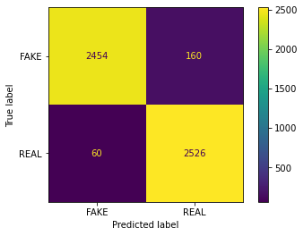
\includegraphics[width=6cm]{imagenes/matriz1.png}}}%
    \qquad
    \subfloat[Algoritmo Pasivo-Agresivo]
    {{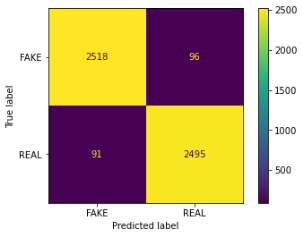
\includegraphics[width=6cm]{imagenes/matriz2.png}}}%
    \caption{Matrices de confusión}%
    \label{fig: confusion}%
\end{figure}

La diagonal principal contiene la suma de todas las predicciones correctas 
(es decir, las noticias que son falsas y reales), mientras que la otra diagonal
refleja los errores del clasificador (falsos positivos y falsos negativos). 
Podemos notar que en este caso, el algoritmo pasivo-agresivo logró obtener 
más predicciones correctas y menos clasificaciones erróneas que el perceptrón 
multicapa. 
\subsection{Reportes de clasificación}

Los reportes de clasificación muestran las principales métricas de clasificación,
incluidas la precisión y la recuperación, la puntuación (media armónica de la
precisión y la recuperación) y el soporte (número de observaciones de esa clase 
en el conjunto de entrenamiento).

\begin{figure}[ht]
    \centering
    \subfloat[MLP]
    {{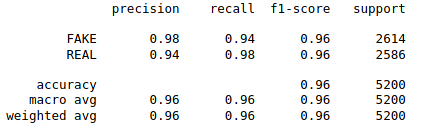
\includegraphics[width=8.5cm]{imagenes/tabla1.png}}}
    \qquad
    \subfloat[Algoritmo Pasivo-Agresivo]
    {{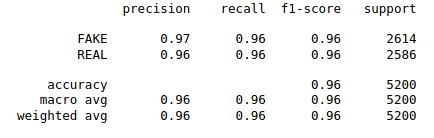
\includegraphics[width=8.5cm]{imagenes/tabla2.png}}}
    \caption{Reportes de clasificación}
    \label{fig: reportes}
\end{figure}

Podemos notar en este caso que el perceptrón multicapa logró una mayor precisión
al clasificar noticias falsas, mientras que el algoritmo pasivo-agresivo logró 
una mayor precisión al clasificar noticas reales. 

En particular, el algoritmo pasivo-agresivo logró un mayor \textit{balance} en 
cuanto a las precisiones al momento de realizar la clasificación binaria. 

\subsection{¡Manos a la obra!}

Ahora bien, veamos cómo funciona cada uno de nuestros modelos al momento de
realizar la clasificación.

\subsubsection{Conjunto de Datos}

Los datos contenidos en el archivo \textit{test.csv} se pueden ver de la 
siguiente forma:
\begin{figure}[ht]
    \centering
    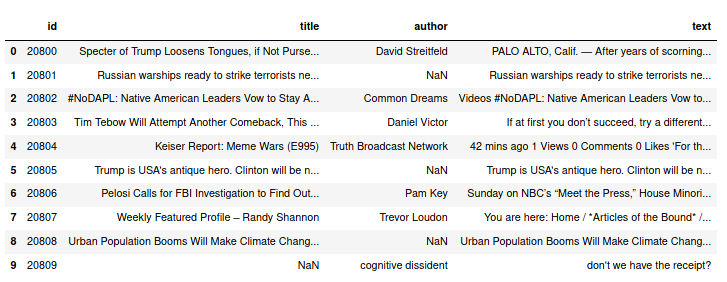
\includegraphics[width=0.8\textwidth]{imagenes/dataframe2.png}
    \caption{DataFrame con las 10 primeras noticias}
    \label{fig: dataframe2}
\end{figure}

\subsubsection{Predicciones}

Una vez que transformamos los datos (igual que transformamos el conjunto de 
prueba anteriormente) y predecimos sobre éstos, obtenemos los siguientes 
resultados:

\begin{figure}[ht]
    \centering
    \subfloat[MLP]
    {{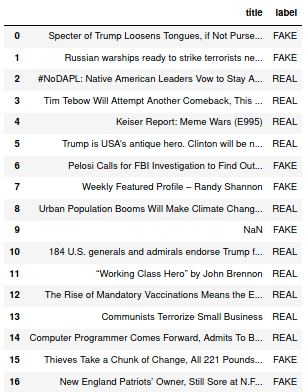
\includegraphics[width=7cm]{imagenes/test1.png}}}
    \qquad
    \subfloat[Algoritmo Pasivo-Agresivo]
    {{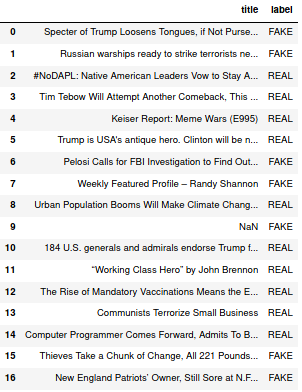
\includegraphics[width=7cm]{imagenes/test2.png}}}
    \caption{DataFrame con las primeras 16 noticias}
\end{figure}

Podemos notar que no existe alguna discrepancia entre ambas clasificaciones, 
al menos para los primeros datos (se hizo la prueba con un conjunto de 50
noticias y aún no encontrábamos diferencias). Para mayor simplicidad sólo 
se mostraron $16$ noticias clasificadas, pero los demás se pueden comprobar 
en el \textit{notebook} que contiene todo el código.

\section{Conclusiones}

Ambos \textit{modelos de clasificación} son bastante buenos. La precisón que 
obtuvo cada uno de ellos superó mis expectativas, ya que no creí que fuera a 
superar el $90\%$. Como no hay que volver a implementar ya sea el perceptrón 
multicapa o el algoritmo de clasificación pasivo-agresivo, me parecen modelos 
bastantes buenos para clasificar grandes cantidades de datos. Personalmente
preferiría el algoritmo pasivo-agresivo si nuestro conjunto de datos fuera 
mucho más grande, ya que este algoritmo es bastante rápido (frente al 
perceptrón) y nos podría dar una excelente clasificación \textit{eficientemente}.

Mi principal problema al momento de elaborar el proyecto fue que no sabía cómo 
preprocesar los datos, pero después de leer un poco sobre el manejo de textos
en \textsc{Python} logré tener un panorama más amplio y me apoyé de las 
herramientas que nos proporciona el lenguaje para \textit{vectorizar} la 
información.

Respecto al proyecto en general, siento que la elección del tema fue bastante 
acertada. Leer sobre las \textit{fake news} me dio mucho qué pensar, es decir, 
sabía que existían pero no sabía a ciencia cierta por qué existían (había 
escuchado brevemente sobre la repercusión que tiene a nivel político). Encontré
 mucho material que aborda el por qué son malas las noticias falsas, en que nos 
pueden afectar y cómo identificarlas. Creo que esto es un tema que nos debería 
preocupar bastante ya que a veces con tanta información ya no sabemos lo que es 
verdad o no (en mi caso, a veces me siento confundida con tantos datos). Es 
importante que entre tanta información forjemos un criterio propio, y defendamos 
lo que para nosotros es \textit{la verdad}, sin olvidar tener fuentes confiables 
con las que sustentar la información que compartimos y respetando siempre a las 
demás personas. 

\begin{thebibliography}{9} 
    \bibitem{1} 
    BB Noticias: Fake News \\
    \url{https://www.bbc.com/mundo/noticias-37910450}

    \bibitem{2}
    ColombiaCheck \\ 
    \url{https://colombiacheck.com/investigaciones/explicador-que-son-las-noticias-falsas}

    \bibitem{3}
    Xataka \\ 
    \url{https://www.xataka.com/otros/13-noticias-falsas-que-hemos-ayudado-a-difundir-por-internet-en-2015}

    \bibitem{4}
    Kaggle: Fake News Dataset \\ 
    \url{https://www.kaggle.com/c/fake-news/data}

    \bibitem{5}
    Passive-Aggressive Algorithm \\ 
    \url{https://www.bonaccorso.eu/2017/10/06/ml-algorithms-addendum-passive-aggressive-algorithms/?subscribe=success#blog_subscription-2}

    \bibitem{6}
    Text classification with Python and Scikit-Learn \\ 
    \url{https://stackabuse.com/text-classification-with-python-and-scikit-learn/}

    \bibitem{7}
    Scikit-Learn: Working with text data \\ 
    \url{https://scikit-learn.org/stable/tutorial/text_analytics/working_with_text_data.html}

    \bibitem{8}
    Kavita Ganesan: Tfidtransformer and TfidVectorizer: usage and differences \\
    \url{https://kavita-ganesan.com/tfidftransformer-tfidfvectorizer-usage-differences/}

    \bibitem{9}
    LUCA: Matriz de confusión \\
    \url{https://empresas.blogthinkbig.com/ml-a-tu-alcance-matriz-confusion/}

    \bibitem{10}
    Koldopina: Matriz de confusión \\
    \url{https://koldopina.com/matriz-de-confusion/}

    \bibitem{11}
    Wikipedia: Tf-idf \\ 
    \url{https://es.wikipedia.org/wiki/Tf-idf}
\end{thebibliography}
\end{document}
